% Encoding: UTF-8
%%%%%%%%%%%%%%%%%%%%%%%%%%%%%%%%%%%%%%%%%%%%%%%%%%%%%%%%%%%%%%%%%%%%%%%%%%%%%%%%

\documentclass{sikthesis}
%\documentclass[draft]{sikthesis}

\usepackage{textcomp} % spezielle Zeichen fuer den Text, z.B. \textmu
\usepackage{algpseudocode} % Pseudocode
\usepackage{booktabs} % Tabellen


% Fuegen Sie hier ggf. weitere benoetigte Pakete ein


%%%%%%%%%%%%%%%%%%%%%%%%%%%%%%%%%%%%%%%%%%%%%%%%%%%%%%%%%%%%%%%%%%%%%%%%%%%%%%%%

% Fuegen Sie hier ggf. weitere ben"otigte tikz-Bibliotheken ein
\usetikzlibrary{automata,positioning}

%%%%%%%%%%%%%%%%%%%%%%%%%%%%%%%%%%%%%%%%%%%%%%%%%%%%%%%%%%%%%%%%%%%%%%%%%%%%%%%%

%\clubpenalty=10000  
%\widowpenalty=10000

%%%%%%%%%%%%%%%%%%%%%%%%%%%%%%%%%%%%%%%%%%%%%%%%%%%%%%%%%%%%%%%%%%%%%%%%%%%%%%%%

% Falls Sie noch weitere Kommandos benoetigen, so ist hier der
% richtige Punkt, diese zu definieren

%%%%%%%%%%%%%%%%%%%%%%%%%%%%%%%%%%%%%%%%%%%%%%%%%%%%%%%%%%%%%%%%%%%%%%%%%%%%%%%%

% Akronyme

\DeclareAcronym{os}{	
  short = OS,
  long = operating system
}


%%%%%%%%%%%%%%%%%%%%%%%%%%%%%%%%%%%%%%%%%%%%%%%%%%%%%%%%%%%%%%%%%%%%%%%%%%%%%%%%
\begin{document}
%%%%%%%%%%%%%%%%%%%%%%%%%%%%%%%%%%%%%%%%%%%%%%%%%%%%%%%%%%%%%%%%%%%%%%%%%%%%%%%%

\frontmatter
% Der allgemeine Anfangsteil der Arbeit wird mit roemischen Zahlen
% nummeriert. Die einzelnen Kapitel im Anfangsteil werden ins
% Inhaltsverzeichnis aufgenommen, erhalten aber keine Nummern

% Tragen Sie hier die Daten f"ur die Titelseite ein
\sikType{Bachelorarbeit} % Art der Arbeit (Diplom/Bachelor/Master)
\sikAuthor{Ho Son Thuy Truong} % Ihr Name
\sikTitle{Automatized Eigensolver for General One-body Potentials} % Titel der Arbeit
\sikMatnr{2020659}
\sikRefereeOne{Prof. Dr. Jakob Kottmann} % Erstgutachter (= betreuender Prof.)
\sikRefereeTwo{Prof. Dr. Mónica Benito} % Zweitgutachter
\sikAdviser{Prof. Dr. Jakob Kottmann} % Betreuer am Lehrstuhl
\sikDate{\today} % Abgabedatum

\sikTitlePage

\chapter*{Abstract}

%%%%%%%%%%%%%%%%%%%%%%%%%%%%%%%%%%%%%%%%%%%%%%%%%%%%%%%%%%%%%%%%%%%%%%%%%%%%%%%%
With quantum dots being a popular research topic following the 2023 Nobel Prize in Chemistry, the need to solve the Schrödinger equation for quantum dots has become increasingly important. 
In this thesis, an automatized eigensolver for general one-body potentials is developed and an example of the harmonic oscillator is demonstrated.
The basis functions for the eigensolver are generated using two different approaches. 
The first method uses the basis functions of the harmonic oscillator to generate the initial guesses, while the second method uses the given potential. In this approach the basis functions depend on the potential.
The eigensolver with general basis functions is tested with different potentials such as Gaussian potentials and double-well potentials.
After generating the basis functions, the convergence between these two methods is compared in terms of speed and accuracy.
This automatized eigensolver is written using MADNESS which ensures a high level of performance and accuracy.


% Inhaltsverzeichnis
\tableofcontents

\mainmatter
% Nun beginnt die eigentliche Arbeit, die Seiten werden hier nun mit
% arabischen Zahlen nummeriert

% Durch das Ablegen jedes Kapitels in einer eigenen Datei bleibt es
% einfacher, die Uebersicht zu behalten
\chapter{Introduction}
\label{c:introduction}


\chapter{Eigensolver for General One-body Potentials}
\label{c:inhalt}

%%%%%%%%%%%%%%%%%%%%%%%%%%%%%%%%%%%%%%%%%%%%%%%%%%%%%%%%%%%%%%%%%%%%%%%%%%%%%%%%


Bei ihrer Abschlussarbeit handelt es sich um eine
  wissenschaftliche Arbeit, die auch entsprechenden
  Qualit"atsanspr"uchen gen"ugen muss.
  \begin{itemize}
  \item Verwenden Sie keine umgangssprachlichen Formulierungen.
  \item Achten Sie darauf, alle Aussagen, die Sie machen, durch
    entsprechende Argumente oder Literaturverweise zu untermauern.
  \item F"uhren Sie vor der Abgabe eine Rechtschreibpr"ufung durch.
    Ein g"angiges Werkzeug hierf"ur ist beispielsweise
    \texttt{aspell}, dessen Verwendung auch in Editoren wie Emacs
    vorgesehen ist.
  \end{itemize}


Kleiner Test ob das Komplieren funktioniert
\section{Methods for Eigensolver}
\section{Approaches to generate Basis Sets}

\section{Basis Set Functions for Harmonic Oscillator}
\section{Basis Set Functions for general Potentials}
\subsection{General Basis Set Functions}
\subsection{Examples}
%\chapter{Kurze Einf"uhrung in \LaTeX}
\label{c:latex}

%%%%%%%%%%%%%%%%%%%%%%%%%%%%%%%%%%%%%%%%%%%%%%%%%%%%%%%%%%%%%%%%%%%%%%%%%%%%%%%%

%%%%%%%%%%%%%%%%%%%%%%%%%%%%%%%%%%%%%%%%%%%%%%%%%%%%%%%%%%%%%%%%%%%%%%%%%%%%%%%%
%%%%%%%%%%%%%%%%%%%%%%%%%%%%%%%%%%%%%%%%%%%%%%%%%%%%%%%%%%%%%%%%%%%%%%%%%%%%%%%%

\section{Gliederung}

%%%%%%%%%%%%%%%%%%%%%%%%%%%%%%%%%%%%%%%%%%%%%%%%%%%%%%%%%%%%%%%%%%%%%%%%%%%%%%%%

Gliedern Sie Ihre Arbeit durch Verwendung von Kapitel
(\verb+\chapter+), Abschnitten (\verb+\section+) und Unterabschnitten
(\verb+\subsection+ und \verb+\subsubsection+). Falls diese nicht
ausreichen, k"onnen Sie auch noch Paragraphen (\verb+\paragraph+)
verwenden. Bei der hier verwendeten Vorlage werden bis zur
Gliederungsstufe \texttt{subsection} automatisch die
Gliederungsnummern erzeugt und entsprechende Eintr"age im
Inhaltsverzeichnis angelegt. Falls sie dies an bestimmten Stellen
nicht w"unschen, verwenden Sie die *-Form des Befehls.

%%%%%%%%%%%%%%%%%%%%%%%%%%%%%%%%%%%%%%%%%%%%%%%%%%%%%%%%%%%%%%%%%%%%%%%%%%%%%%%%
%%%%%%%%%%%%%%%%%%%%%%%%%%%%%%%%%%%%%%%%%%%%%%%%%%%%%%%%%%%%%%%%%%%%%%%%%%%%%%%%

\section{Textgestaltung}

%%%%%%%%%%%%%%%%%%%%%%%%%%%%%%%%%%%%%%%%%%%%%%%%%%%%%%%%%%%%%%%%%%%%%%%%%%%%%%%%

\LaTeX~ bietet verschiedene M"oglichkeiten, einen Text zu
strukturieren. Die folgenden Abschnitte zeigen kurz die Verwendung von
Aufz"ahlungen, Tabellen und Bildern.

%%%%%%%%%%%%%%%%%%%%%%%%%%%%%%%%%%%%%%%%%%%%%%%%%%%%%%%%%%%%%%%%%%%%%%%%%%%%%%%%

\subsection{Aufz"ahlungen}

In \LaTeX~ gibt es drei Arten von Aufz"ahlungen. Wohl am h"aufigsten
verwendet wird die \texttt{itemize}-Umgebung:
\begin{itemize}
\item Das ist der erste Aufz"ahlungspunkt.
\item noch ein Aufz"ahlungspunkt.
\item Aufz"ahlungen k"onnen selbstverst"andlich auch aus l"angeren und
  mehreren Textabschnitten bestehen. \LaTeX~ k"ummert sich dann wie im
  normalen Flie"stext um den korrekten Satz des Aufz"ahlungstextes.
\end{itemize}

Manchmal m"ochte man Aufz"ahlungen nummerieren. Dazu wird die
\texttt{enumerate}-Umgebung verwendet:
\begin{enumerate}
\item Einzelne Aufz"ahlungspunkte werden auch hier mittels
  \verb+\item+ gesetzt.
\item Die Nummerierung wird von LaTeX automatisch erzeugt.
\item Aufz"ahlungen k"onnen auch geschachtelt werden:
  \begin{itemize}
  \item Hier mit einer nicht nummerierten Aufz"ahlung.
  \end{itemize}
\end{enumerate}

Falls Sie mehrere Begriffe erkl"aren m"ochten, bietet sich die
\texttt{description}-Umgebung an:
\begin{description}
\item[Verwendung] Descriptions werden wie alle anderen Aufz"ahlungen
  gesetzt. Denken Sie aber daran, dem \verb+\item+ als Option den zu
  beschreibenden Begriff mitzugeben.
\item[Textauszeichnung] Sie k"onnen einzelne Textteile mittels
  \verb+\textXX+ auch in \textbf{fett}, \textit{kursiv} oder
  \textsc{Small Caps} setzen, um diese Hervorzuheben. F"ur einfache
  Hervorhebungen sollten Sie aber besser das \verb+\emph+-Kommando
  \emph{benutzen}, da dieses auch geschachtelt werden kann.
\item[Dokumentenklasse] Der erste Befehl eines \LaTeX-Dokuments legt
  die Dokumentenklasse (verwendete Vorlage) fest. Dieses Dokument
  verwendet z.B. die Klasse \texttt{sikthesis}
  (\verb+\documentclass{sikthesis}+). Sie k"onnen der Dokumentenklasse
  ein optionales Argument \verb+[draft]+ mitgeben, um einen Entwurf
  des Dokuments zu erzeugen. Bilder werden dann nur als leere Rahmen
  angezeigt, und \LaTeX~ markiert Stellen am Rand, in denen noch
  Probleme beim Umbruch bzw. mit "uberlangen Texten bestehen. Diese
  Probleme lassen sich im Allgemeinen durch geringf"ugiges
  Umformulieren des Textes beheben.
\end{description}

%%%%%%%%%%%%%%%%%%%%%%%%%%%%%%%%%%%%%%%%%%%%%%%%%%%%%%%%%%%%%%%%%%%%%%%%%%%%%%%%

\subsection{Tabellen}

Eine Tabelle wird in \LaTeX~ mittels der \texttt{tabular}-Umgebung
erzeugt und in  \texttt{table}-Umgebungen eingebettet. \LaTeX platziert diese Tabellen dann \emph{flie"send}. Solche
Tabellen sollten mit einer \verb+\caption+ versehen und
ggf. im Text referenziert werden (siehe Tabelle \ref{t:beispiel}).
Falls der \verb+\caption+-Text sehr lang ist, empfiehlt es sich, dem
Makro noch einen Kurztext f"ur das Tabellenverzeichnis als optionales
Argument zu geben:
\verb+\caption[Text fuer Tabellenverzeichnis]{Beschriftung}+.


\begin{table}[h]
\begin{center}
\caption{Tabellenüberschrift}\label{t:beispiel}
\begin{tabular}{rcccccccccccc}
\toprule
  a & b & c\\
\midrule
1 & 2 & 333333333\\
1 & 2 & 3333333333\\
\midrule
1 & 2 & 3333333333\\
1 & 2 & 3333333333\\
\bottomrule
\end{tabular}
\end{center}
\end{table}

%%%%%%%%%%%%%%%%%%%%%%%%%%%%%%%%%%%%%%%%%%%%%%%%%%%%%%%%%%%%%%%%%%%%%%%%%%%%%%%%

\subsection{Grafiken}

Wie auch Tabellen sollten Grafiken flie"send gesetzt werden, so dass
sich m"oglichst \LaTeX um deren Platzierung k"ummert. Abbildung
\ref{f:beispiel} zeigt ein Beispiel f"ur ein solches Bild.
Dabei wird das Makro \verb+\missingfigure{...}+ aus dem Paket
\verb+todonotes+ als Platzhalter f"ur eine Grafik verwendet.

\begin{figure}[htbp]
  \centering
  %\includegraphics[width=0.6\textwidth]{unilogo-b}
  \missingfigure{Beispielbild}
  \caption[Kurzbeschreibung f"ur die listoffigures]{Beispiel f"ur ein
    Bild, 60\% Textbreite, die Breite kann aber auch absolut angegeben
    werden, z.B. 6cm}
  \label{f:beispiel}
\end{figure}

Nutzen Sie zur Erstellung von Grafiken m"oglichst das Paket \tikz.
Dabei geben Sie die Beschreibung der Grafik direkt im \TeX-Code an.
Damit wird insbesondere sichergestellt, dass Beschriftungen in der
Grafik das gleich Schriftbild haben wie der Text Ihrer Arbeit.
Ein Beispiel f"ur eine solche Grafik finden Sie in den
Abbildungen~\ref{f:tikz1} und \ref{f:tikz2}.
Diese Abbildungen zeigen auch, wie Sie zwei Grafiken mittels
\verb+minipage+-Umgebungen nebeneinander platzieren k"onnen.

\begin{figure}[htbp]
  \begin{minipage}{0.5\textwidth}
    \centering
    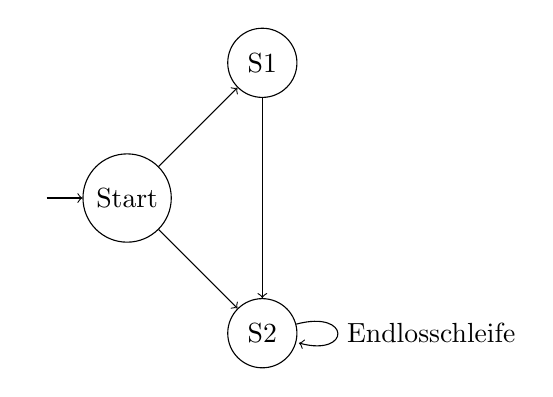
\begin{tikzpicture}[initial text={}]
      \node [state,initial] (start) {Start};
      \node [state,above right=of start] (s1) {S1};
      \node [state,below right=of start] (s2) {S2};
      \path [->]
      (start) edge (s1)
      (start) edge (s2)
      (s1) edge (s2)
      (s2) edge [loop right] node [right] {Endlosschleife} ();
    \end{tikzpicture}
    \caption{\tikz-Grafik 1}
    \label{f:tikz1}
  \end{minipage}
  %
  \begin{minipage}{0.5\textwidth}
    \centering
    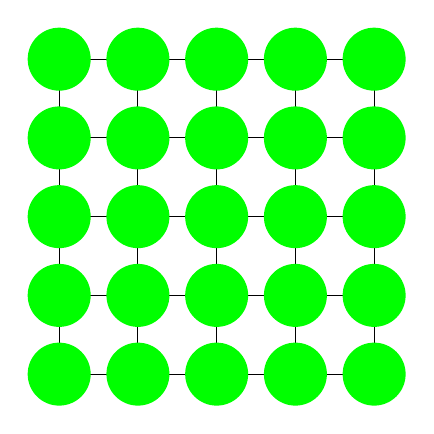
\begin{tikzpicture}
      \draw (0,0) grid (4,4);
      \foreach \x in {0,1,...,4} {
        \foreach \y in {0,1,...,4} {
          \fill [green] (\x,\y) circle (0.4cm);
        }
      }
    \end{tikzpicture}
    \caption{\tikz-Grafik 2}
    \label{f:tikz2}
  \end{minipage}
\end{figure}

Zur Erstellung von Diagrammen k"onnen Sie das Paket \verb+pgfplots+
verwenden, das auf \tikz bzw. PGF basiert.
Beispiele hierf"ur finden Sie in den Abbildungen~\ref{f:pgf1} und
\ref{f:pgf2}.

\begin{figure}[htbp]
  \begin{minipage}{0.5\textwidth}
    \centering
    \begin{tikzpicture}
      \begin{axis}[
          width=0.8\textwidth,
          %ybar,
          %bar width=0.1cm,
          ylabel={Execution time (cycles)},
          xlabel={Core},
          legend style={at={(0.5,1.05)},anchor=south,legend
            columns=-1}
        ]
        
        %fullimg
        \addplot +[only marks,mark=+] coordinates {
          (0,770865)
          (1,329608)
          (2,550254)
          (3,770900)
        };
        
        %nokrep
        \addplot +[only marks,mark=x] coordinates {
          (0,693448)
          (1,369585)
          (2,531878)
          (3,694171)
        };
        
        %mossca
        \addplot +[only marks,mark=*] coordinates {
          (0,686010)
          (1,361362)
          (2,523655)
          (3,685948)
        };
        
        \legend{FI,SI,SD}
      \end{axis}
    \end{tikzpicture}
    
    \caption{pgf-Diagramm 1}
    \label{f:pgf1}
  \end{minipage}
  %
  \begin{minipage}{0.5\textwidth}
    \centering
    
    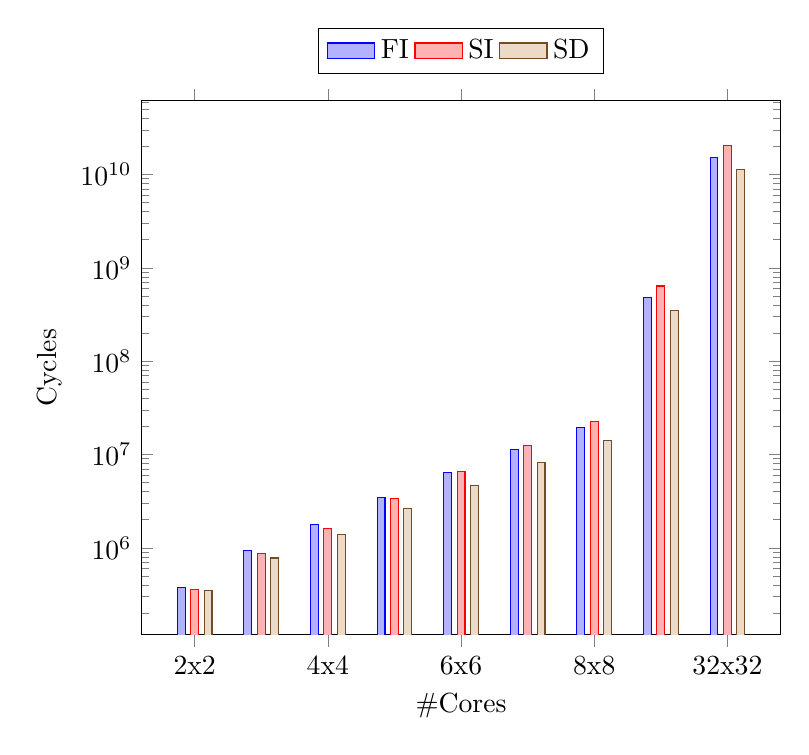
\begin{tikzpicture}
      \begin{semilogyaxis}[
          width=0.8\textwidth,
          ybar,
          bar width=0.1cm,
          ylabel={Cycles},
          xlabel={\#Cores},
          legend style={at={(0.5,1.05)},anchor=south,legend
            columns=-1},
          symbolic x coords={2x2,3x3,4x4,5x5,6x6,7x7,8x8,16x16,32x32}
        ]
        
        %fullimg
        \addplot +[area legend] coordinates {
          (2x2, 376662) (3x3, 946144) (4x4, 1794265) (5x5, 3470767) (6x6, 6352207) (7x7, 11348627) (8x8, 19489997) (16x16, 481008057) (32x32, 15336870167)
        };
        %nokrep
        \addplot +[area legend] coordinates {
          (2x2, 360174) (3x3, 861960) (4x4, 1628092) (5x5, 3382747) (6x6, 6623068) (7x7, 12603816) (8x8, 22750681) (16x16, 637517992) (32x32, 20568322109)
        };
        %mossca
        \addplot +[area legend] coordinates {
          (2x2, 349798) (3x3, 778817) (4x4, 1402881) (5x5, 2609504) (6x6, 4655134) (7x7, 8225318) (8x8, 14110261) (16x16, 349710481) (32x32, 11253110760)
        };
        \legend{FI,SI,SD}
      \end{semilogyaxis}
    \end{tikzpicture}
    \caption{pgf-Diagramm 2}
    \label{f:pgf2}
  \end{minipage}
\end{figure}

%%%%%%%%%%%%%%%%%%%%%%%%%%%%%%%%%%%%%%%%%%%%%%%%%%%%%%%%%%%%%%%%%%%%%%%%%%%%%%%%
%%%%%%%%%%%%%%%%%%%%%%%%%%%%%%%%%%%%%%%%%%%%%%%%%%%%%%%%%%%%%%%%%%%%%%%%%%%%%%%%

\section{Satz von mathematischen Symbolen}

%%%%%%%%%%%%%%%%%%%%%%%%%%%%%%%%%%%%%%%%%%%%%%%%%%%%%%%%%%%%%%%%%%%%%%%%%%%%%%%%

Mathematische Formeln im Text werden mittels \$-Zeichen
gekennzeichnet, z.B. $E=mc^2$. Abgesetzte Formeln werden
folgenderma"sen gesetzt:
\[f(x) = \frac{1}{\sigma\sqrt{2\pi}}
\exp\left(-\frac{(x-\mu)^2}{2\sigma^2}\right)\]
Falls sie Formeln nummerieren m"ochten, verwenden Sie die
\texttt{equation}-Umgebung:
\begin{equation}
  \label{eq:nd}
F(x) = \frac{1}{\sigma\sqrt{2\pi}} \int_{-\infty}^x
\exp\left(-\frac{(t-\mu)^2}{2\sigma^2}\right)\,dt
\end{equation}
Nun kann die Formel im Text mittels \verb+\eqref+ referenziert werden:
Gleichung~\eqref{eq:nd}.

Beachten Sie, dass \LaTeX~ im mathematischen Modus jedes Zeichen als
eigene Variable ansieht.
Die Zeichenkette $size$ wird also als Produkt der Variablen $s$, $i$,
$z$ und $e$ gesetzt (auf die Angabe des Multiplikationszeichen wird
meistens verzichtet).
Falls Sie stattdessen eine Variable mit einem l"angeren Namen
verwenden m"ochten, setzen Sie diesen mit \verb+\mathit{...}+,
z.B. $\mathit{size}$.
Wenn Sie genau hinsehen, erkennen Sie, dass in diesem Fall die
Zeichenabst"ande anders gesetzt werden.

%%%%%%%%%%%%%%%%%%%%%%%%%%%%%%%%%%%%%%%%%%%%%%%%%%%%%%%%%%%%%%%%%%%%%%%%%%%%%%%%
%%%%%%%%%%%%%%%%%%%%%%%%%%%%%%%%%%%%%%%%%%%%%%%%%%%%%%%%%%%%%%%%%%%%%%%%%%%%%%%%

\section{Externe Referenzen}

%%%%%%%%%%%%%%%%%%%%%%%%%%%%%%%%%%%%%%%%%%%%%%%%%%%%%%%%%%%%%%%%%%%%%%%%%%%%%%%%

Literaturverweise werden mittels BibTeX verwaltet. Dazu werden die
Referenzen in einer eigenen Datei abgelegt (z.B. \texttt{thesis.bib})
und mit K"urzeln versehen. Diese k"onnen dann im Text referenziert
werden. Beachten Sie, dass sie Ihr Dokument nun zweimal "ubersetzen
m"ussen. Zwischen den beiden \texttt{latex}-
bzw. \texttt{pdflatex}-Aufrufen m"ussen Sie \texttt{bibtex}
aufrufen. Weitere Informationen hierzu und zur Verwendungen von
\LaTeX~ im Allgemeinen finden Sie in \cite{kopka} sowie im Internet.

%%%%%%%%%%%%%%%%%%%%%%%%%%%%%%%%%%%%%%%%%%%%%%%%%%%%%%%%%%%%%%%%%%%%%%%%%%%%%%%%
%%%%%%%%%%%%%%%%%%%%%%%%%%%%%%%%%%%%%%%%%%%%%%%%%%%%%%%%%%%%%%%%%%%%%%%%%%%%%%%%

\section{Helfer}

%%%%%%%%%%%%%%%%%%%%%%%%%%%%%%%%%%%%%%%%%%%%%%%%%%%%%%%%%%%%%%%%%%%%%%%%%%%%%%%%

In dieser Vorlage sind noch weitere Pakete eingebunden, die Ihnen das
Arbeiten mit \LaTeX und Erstellen Ihrer Abschlussarbeit erleichtern
sollen:
\begin{description}
\item[acro] erm"oglicht die bequeme Verwendung von Abk"urzungen, ohne
  dass Sie selbst verfolgen m"ussen, ob diese an einer bestimmten
  Stelle bereits verwendet wurden.
  Mittels \verb+\DeclareAcronym{id}{short=...,long=...}+ im Vorspann des Dokuments k"onnen die
  Akromyme definiert werden.
  Im Text wird das Akronym dann mittels \verb+\ac{id}+ verwendet.
  Bei der ersten Verwendung wird dabei die Langbezeichnung mit
  Abk"urzung erzeugt, wie beispielsweise in \glqq\ac{os}\grqq, bei
  sp"aterer Verwendung wird nur noch die Kurzschreibweise
  ausgegegeben, also \glqq\ac{os}\grqq.
  Eine Liste aller vorhandenen Akronyme erzeugen Sie mit \verb+\printacronyms+.
\item[todonotes] sind f"ur die laufende Arbeit am Dokument hilfreich.
  Hiermit lassen sich Randnotizen erzeugen, die z.B. Hinweise f"ur die
  sp"atere "Uberarbeitungen enthalten.
  \todo{Beispiel f"ur eine Todonote}
  Au"serdem k"onnen mit diesem Paket auch Platzhaltergrafiken wie in
  Abb.~\ref{f:beispiel} erstellt werden.
  Mittel \verb+\todototoc+ k"onnen Sie sich eine Liste aller
  vorhandenen Todo-Notizen erzeugen lassen.
\end{description}

%%%%%%%%%%%%%%%%%%%%%%%%%%%%%%%%%%%%%%%%%%%%%%%%%%%%%%%%%%%%%%%%%%%%%%%%%%%%%%%%
%%% Local Variables: 
%%% mode: latex
%%% TeX-master: thesis
%%% TeX-PDF-mode: t
%%% End: 
%%%%%%%%%%%%%%%%%%%%%%%%%%%%%%%%%%%%%%%%%%%%%%%%%%%%%%%%%%%%%%%%%%%%%%%%%%%%%%%%
%<!-- Local IspellDict: german -->

\chapter{Results}
\label{c:results}

%%%%%%%%%%%%%%%%%%%%%%%%%%%%%%%%%%%%%%%%%%%%%%%%%%%%%%%%%%%%%%%%%%%%%%%%%%%%%%%%





\chapter{Conclusion}
\label{c:conclusion}

% Verzeichnisse

%\listoffigures
%\listoftables
\bibliographystyle{abbrv}
\bibliography{thesis}

% Falls noetig, koennen Sie hier noch Anhaenge aufnehmen. Die
% Anhangskapitel werden mit Buchstaben nummeriert. Auch hier sollte
% jedes Kapitel in einer eigenen Datei liegen.

%\begin{appendix}
%\chapter{Anhangskapitel}
%Falls Sie noch Informationen in die Arbeit einfügen m"ochten, die nur
%am Rande relevant für das Verst"andnis Ihrer Arbeit sind, so legen
%Sie daf"ur einen Anhang an.
%Internetreferenz \cite{heise}, Referenz mit mehreren Autoren \cite{liu73acm}
%\section{foo}
%\section{bar}
%\chapter{Zweites Anhangskapitel}
%\end{appendix}

\backmatter

\end{document}
